\documentclass[12pt]{article}
\usepackage{preamble}
\usepackage{longtable}

\geometry{a4paper, left=2.5cm, right=2.5cm, top=2cm, bottom=2.5cm}

\pagestyle{plain}

\newcommand{\placeholder}[1]{{\color{magenta}#1}}

\chead{
    \begin{minipage}{1\linewidth}
        \begin{wrapfigure}{r}{0pt}
            \includegraphics[height=1cm]{images/logo}
        \end{wrapfigure}
        {
            \centering
            \sffamily\scriptsize
            \textbf{
                Санкт-Петербургский национальный исследовательский университет \\
                информационных технологий, механики и оптики}
            %th3p4g
            \vspace{2mm}

            \quad\quad\quad\quad\quad\quad\ \textbf{УЧЕБНЫЙ ЦЕНТР ОБЩЕЙ ФИЗИКИ ФТФ}
        }
    \end{minipage}
}



\begin{document}
    \vspace*{2\baselineskip}

    \thispagestyle{fancy}

    \noindent
    \textbf{Группа} \underline{\hspace{4.85cm}} \hfill \textbf{К работе допущен} \underline{\hspace{4cm}} \\[0.5cm]
    \textbf{Студент} \underline{\hspace{4.6cm}} \hfill \textbf{Работа выполнена} \underline{\hspace{4cm}} \\[0.5cm]
    \textbf{Преподаватель} \underline{\hspace{3.2cm}} \hfill \textbf{Отчет принят} \underline{\hspace{4.85cm}} \\


    \begin{center}
    {\huge \textbf{Рабочий протокол и отчёт по\\ лабораторной работе № 1.04}}

        \smallvspace

        {\Large Исследование равноускоренного вращательного движения (маятник Обербека)}
    \end{center}


    \noindent
    1. \textbf{Цель работы.}

    \begin{enumerate}
        \item Проверка основного закона динамики вращения.

        \item Проверка зависимости момента инерции от положения масс относительно оси вращения
    \end{enumerate}

    \mediumvspace

    \noindent
    2. \textbf{Задачи, решаемые при выполнении работы.}

    \begin{enumerate}
        \item Измерение времени падения груза при разной массе груза и разном положении утяжелителей на крестовине.

        \item Расчёт ускорения груза, углового ускорения крестовины и момента силы натяжения нити.

        \item Расчёт момента инерции крестовины с утяжелителями и момента силы трения.

        \item Исследование зависимости момента силы натяжения нити от углового ускорения.
        Проверка основного закона динамики вращения.

        \item Исследование зависимости момента инерции от положения масс
        относительно оси вращения. Проверка теоремы Штейнера.
    \end{enumerate}

    \mediumvspace

    \noindent
    3. \textbf{Объект исследования} \\
    Маятник Обербека: крестовина с перемещаемыми по спицам грузами-утяжелителями и груз, создающий натяжение нити и раскручивающий крестовину.

    \mediumvspace

    \noindent
    4. \textbf{Метод экспериментального исследования.} \\
    Условные прямые измерения времени падения груза, раскручивающего крестовину.

    \newpage    

    \noindent
    5. \textbf{Рабочие формулы и исходные данные.}

    \begin{center}
    \textbf{Исходные данные}
\end{center}

\begin{flushleft}
    $\text{Масса каретки} \hspace{4.95cm} (47,0 \pm 0,5)\text{г}$ \\
    $\text{Масса шайбы} \hspace{5.2cm} (220,0 \pm 0,5)\text{г}$ \\
    $\text{Масса грузов на крестовине} \hspace{2.45cm} (408,0 \pm 0,5)\text{г}$ \\
    $\text{Расстояние первой риски от оси} \hspace{1.7cm} (57,0 \pm 0,5)\text{мм}$ \\
    $\text{Расстояние между рисками} \hspace{2.55cm} (25,0 \pm 0,2)\text{мм}$ \\
    $\text{Диаметр ступицы} \hspace{4.35cm} (46,0 \pm 0,5)\text{мм}$ \\
    $\text{Диаметр груза на крестовине} \hspace{2.15cm} (40,0 \pm 0,5)\text{мм}$ \\
    $\text{Высота груза на крестовине} \hspace{2.4cm} (40,0 \pm 0,5)\text{мм}$ \\
\end{flushleft}

\begin{center}
    \textbf{Рабочие формулы}
\end{center}

\text{Ускорение груза}
\[
a = \frac{2h}{t^2}
\]
Где:
\[
\text{$h$ - расстояние, пройденное грузом за время $t$ от начала движения}
\]

\text{Связь между угловым ускорением и линейным ускорением груза} 
\[
\varepsilon = \frac{2a}{d} = \frac{4h}{t^2d}
\]
Где:
\[
\text{$d$ — диаметр ступицы}
\]

\text{Момент силы натяжения нити}
\[
M = \frac{m d}{2} \left(g - a \right) = \frac{m d}{2} \left(g - \frac{2 h}{t^2} \right)
\]

\text{Основной закон динамики вращения}
\[
I \varepsilon = M - M_{\text{тр}}
\]
Где:
\begin{center}
    \text{$I$ — момент инерции крестовины} \\
    \text{$\varepsilon$ — угловое ускорение крестовины} \\
    \text{$M$ и $M_{\text{тр}}$ — моменты сил натяжения нити и трения на крестовине} \\
\end{center}

\begin{center}
    \text{В соответствии с теоремой Штейнера момент инерции крестовины зависит от расстояния} 
    \text{между центрами грузов и осью вращения по формуле}
\end{center} 
\[
I = I_0 + 4 m_{\text{ут}} R^2
\]
Где:
\begin{center}
    \text{$I_0$ - сумма моментов инерции стрежней крестовины, момента инерции ступицы} 
    \text{и собственных центральных моментов инерции утяжелителей}
\end{center}

\text{Момент инерции крестовины с утяжелителями по МНК} 
\[
I = \frac{\sum_{i=1}^{N} \left( \varepsilon_i - \overline{\varepsilon} \right) \left( M_i - \overline{M} \right)}{\sum_{i=1}^{N} \left( \varepsilon_i - \overline{\varepsilon} \right)^2}
\]

\text{Расстояние от оси крестовины до грузов-утяжелителей}: 
\[
R = l_1 + \left( n - 1 \right) l_0 + \frac{b}{2}
\]

Где:
\begin{center}
    \text{$l_1$ – расстояние от оси вращения до первой риски} \\
    \text{$n$ – номер риски, на которой установлены утяжелители} \\
    \text{$l_0$ – расстояние между соседним рисками} \\
    \text{$b$ – размер утяжелителя вдоль спицы} \\
\end{center}

\text{Момент инерции крестовины по т. Штейнера}
\[
I_0 = \overline{I} - 4m_{\text{ут}}\overline{R}^2
\]
Где:
\[
m_\text{ут} = \frac{\sum_{i=1}^{N} \left( R_i - \overline{R} \right) \left( I_i - \overline{I} \right)}{4\sum_{i=1}^{N} \left( R_i - \overline{R} \right)^2}
\]

\[
\Delta m_{\text{ут}} = \frac{2 \cdot \sqrt{\frac{\sum_{i=1}^{N} \left( I_i - \left( I_0 + 4 m_{\text{ут}} R_i^2 \right) \right)^2}{(N - 2) \sum_{i=1}^{N} \left( R_i^2 - \bar{R}^2 \right)}}}{4} \quad \quad \Delta I_0 = 2 \cdot \sqrt{\left( \frac{1}{N} + \frac{\overline{R}^2}{\sum_{i=1}^{N} \left( R_i^2 - \overline{R}^2 \right)^2} \right) \cdot \frac{\sum_{i=1}^{N} \left( I_i - \left( I_0 + 4 m_{\text{ут}} R_i^2 \right) \right)^2}{N-2}}
\]

\text{Абсолютная погрешность с учетом погрешности приборов}: 
\[
\Delta x = \sqrt{\left( \overline{\Delta x} \right)^2 + \left( \frac{2}{3} \Delta_{\text{ux}} \right)^2}
\]
Где:
\begin{center}
    \text{$\Delta_{\text{ux}}$ — погрешность прибора}
    \text{$\overline{\Delta x}$ — случайная погрешность (доверительный интервал)}
\end{center}

\text{Погрешность косвенного значения}: 
\[
\Delta z = \sqrt{\left( \frac{\partial z}{\partial x_1} \Delta x_1 \right)^2 + \left( \frac{\partial z}{\partial x_2} \Delta x_2 \right)^2}
\]
Где:
\[
z = f(x_1, x_2)
\]

\text{Относительная погрешность}: 
\[
\varepsilon_x = \frac{\Delta x}{\overline{x}} \cdot 100\%
\]


    \mediumvspace

    \noindent
    6. \textbf{Измерительные приборы.}

    \smallvspace

    \begin{center}
    \begin{tabular}{|c|m{5cm}|C{2cm}|C{2cm}|C{2cm}|c|}
        \hline
        № п/п & Наименование               & Предел\newlineизмерений & Цена\newlineделения & Класс\newlineточности & $\Delta_{\text{и}x}$ \\
        \hline
        1     & Секундомер                 & $10$ с                  & $0.01$ с/дел          & \---                   & $0.01$ с     \\
        \hline
        2     & Линейка                    & $0.7$ м                 & $1$ мм/дел          & \---                     & $1$ мм   \\
        \hline
    \end{tabular}

    \smallvspace

    \textit{Таблица 1.} Измерительные приборы
\end{center}

    \mediumvspace

    7. \textbf{Схема установки. (перечень схем, которые составляют Приложение 1).}

    \hyperlink{schema1}{Схема установки} прилагается в Приложении 1

    \mediumvspace

    8. \textbf{Результаты прямых измерений и их обработки.}

    \begin{itemize}
    \item Прилагается \hyperlink{table2}{Таблица 2} в Приложении 2
\end{itemize}


    \mediumvspace

    9. \textbf{Расчет результатов косвенных измерений.}

    \begin{itemize}
    \item Прилагается \hyperlink{table3}{Таблица 3} в Приложении 2
    \item Прилагается \hyperlink{table4}{Таблица 4} в Приложении 2
    \item Прилагается \hyperlink{table5}{Таблица 5} в Приложении 2
    \item Прилагается \hyperlink{table6}{Таблица 6} в Приложении 2

    Расчёт по методу наименьших квадратов $m_\text{ут}$ и $I_0$ \\
    \[
        m_\text{ут} = \frac{\sum_{i=1}^{N} \left( R_i - \overline{R} \right) \left( I_i - \overline{I} \right)}{4\sum_{i=1}^{N} \left( R_i - \overline{R} \right)^2} = 0,4706 \ \text{кг}
    \]
    \[
        I_0 = \overline{I} - 4m_{\text{ут}}\overline{R}^2 = 0,0093 \ \text{кг} \cdot \text{м}^2
    \]
\end{itemize}

    \mediumvspace

    10. \textbf{Расчёт погрешности измерений.}

    \mediumvspace

    11. \textbf{Графики (перечень графиков, которые составляют Приложение 3).}

    \hyperlink{diagram1}{График 1} прилагается в Приложении 3

    \mediumvspace

    12. \textbf{Окончательные результаты.}

    В ходе выполнения работы получаем доверительные интервалы для массы утяжелителя и момента инерции стержней крестовины:

\begin{tabular}{lll}
    $m_{\text{ут}} = (0.471 \pm 0.040) \ \text{кг}$ & $\varepsilon = 8.40\%$ & $\alpha = 0.95$ \\

    $I_0 = (0.0092 \pm 0.0038) \ \text{кг} \cdot \text{м}^2$ & $\varepsilon = 41.59\%$ & $\alpha = 0.95$ \\
\end{tabular}

    \mediumvspace

    13. \textbf{Выводы и анализ результатов работы.}

    В ходе эксперимента были собраны данные для расчета параметров, необходимых для проверки зависимости момента инерции от массы утяжелителей, размещенных на спицах вращающейся крестовины. Эксперимент подтвердил теоретические основы динамики вращательного движения: был проверен закон, связывающий угловое ускорение с моментами сил трения и натяжения нити. \\
Для некоторых характеристик динамики вращения были определены доверительные интервалы, и на основе полученных данных построены соответствующие графики.

    \clearpage

    \begin{center}
        \LARGE
        \textbf{Приложение 1. Схема установки}
    \end{center}

    \mediumvspace

    \input{schema1}

    \clearpage

    \begin{center}
        \LARGE
        \textbf{Приложение 2. Таблицы измерений и расчётов}
    \end{center}

    \mediumvspace

    \begin{center}
    \begin{tabular}{|p{2.3cm}|p{0.5cm}|p{1.5cm}|p{1.5cm}|p{1.5cm}|p{1.5cm}|p{1.5cm}|p{1.5cm}|}
        \hline
        \multirow{2}{2.3cm}{Масса груза, кг} & \multirow{2}{*}{№} & \multicolumn{6}{c|}{Положение утяжелителей} \\
        \cline{3-8}
         & & 1 риска       & 2 риска & 3 риска & 4 риска & 5 риска & 6 риска \\
        \hline
        \multirow{4}{*}{$m_1 = 0.267$} & $t_1$ &    4.79     &     5.73    &     6.81    &    7.87     &   8.69      &     9.92    \\
        \cline{2-8}
        & $t_2$ &   4.90     &     5.82    &     6.88    &     7.67    &     8.52    &    9.43     \\
        \cline{2-8}
        & $t_3$ &   4.87     &     5.68    &     6.68    &     7.48    &    8.50     &    9.78     \\
        \cline{2-8}
        % & $t_\text{ср}$ &  $4,85 \pm 0,14$  &    $5,74 \pm 0,18$     &    $6,79 \pm 0,25$     &    $7,67 \pm 0,48$     &    $8,54 \pm 0,36$     &     $9,71 \pm 0,62$    \\
        & $t_\text{ср}$ &  4.85  &    5.74     &    6.79     &    7.67     &    8.54     &     9.71    \\
        \hline
        \multirow{4}{*}{$m_2 = 0.487$} & $t_1$ &      3.57        &     4.32    &    4.89     &     5.47    &     6.30    &     7.00    \\
        \cline{2-8}
        & $t_2$ &       3.55        &     4.12    &     4.87    &     5.55    &     6.27    &   6.96      \\
        \cline{2-8}
        & $t_3$ &       3.44        &     4.31    &     4.97    &     5.68    &    6.19     &   6.75     \\
        \cline{2-8}
        %& $t_\text{ср}$ &      $3,52 \pm 0,17$         &    $4,25 \pm 0,28$     &    $4,91 \pm 0,13$     &   $5,57 \pm 0,26$      &     $6,25 \pm 0,14$    &     $6,90 \pm 0,33$    \\
        & $t_\text{ср}$ &      3.52         &    4.25     &    4.91    &   5.57      &     6.25    &     6.90    \\
        \hline
        \multirow{4}{*}{$m_3 = 0.707$} & $t_1$ &      3.03        &     3.59    &     3.89    &    4.65     &    5.30     &     5.96    \\
        \cline{2-8}
        & $t_2$ &       2.72        &     3.55    &     4.02    &    4.40     &    5.27     &    5.79     \\
        \cline{2-8}
        & $t_3$ &       2.90        &    3.61     &     3.87    &     4.68    &    5.09     &    5.84     \\
        \cline{2-8}
        %& $t_\text{ср}$ &      $2,88 \pm 0,39$        &    $3,58 \pm 0,08$     &    $3,93 \pm 0,20$     &    $4,58 \pm 0,38$     &    $5,22 \pm 0,28$     &     $5,86 \pm 0,22$    \\
        & $t_\text{ср}$ &      2.88       &    3.58    &    3.93     &    4.58     &   5.22     &     5.86    \\
        \hline
        \multirow{4}{*}{$m_4 = 0.927$} & $t_1$ &      2.39        &     2.86    &     3.55    &    4.20     &    4.39     &     4.90    \\
        \cline{2-8}
        & $t_2$ &       2.50        &    2.92     &    3.52     &    3.89     &    4.67     &    4.98     \\
        \cline{2-8}
        & $t_3$ &       2.70        &    2.85     &    3.48     &    4.12     &    4.59     &     5.12    \\
        \cline{2-8}
        %& $t_\text{ср}$ &      $2,53 \pm 0,39$        &    $2,88 \pm 0,09$     &     $3,52 \pm 0,09$    &    $4,07 \pm 0,40$     &    $4,55 \pm 0,36$     &     $5,00 \pm 0,28$    \\
        & $t_\text{ср}$ &      2.53        &    2.88     &     3.52    &    4.07     &    4.55     &     5.00    \\
        \hline

    \end{tabular}

    \smallvspace

    \textit{Таблица 2.} Протокол измерений времени падения груза при разной
    массе груза и разном положении утяжелителей на крестовине
\end{center}


    \mediumvspace

    \begin{center}
    \begin{tabular}{|p{2.5cm}|p{2cm}|p{2cm}|p{2cm}|p{2cm}|p{2cm}|p{2cm}|}
        \hline
        \multirow{3}{*}{Масса груза} & \multicolumn{6}{c|}{Положение утяжелителей} \\
        \cline{2-7}
        & 1 риска       & 2 риска & 3 риска & 4 риска & 5 риска & 6 риска \\
        \cline{2-7}
        & \multicolumn{6}{c|}{Ускорение $a, \frac{\text{м}}{\text{с}^2}$} \\
        \hline
        $m_1 = 0.267 \text{кг}$ &   0,06    &   0,04    &    0,03   &    0,02   &    0,02   &   0,01    \\
        \hline
        $m_2 = 0.487 \text{кг}$ &   0,11    &   0,08    &    0,06   &    0,05   &    0,04   &   0,03    \\
        \hline
        $m_3 = 0.707 \text{кг}$ &   0,17    &   0,11    &    0,09   &    0,07   &    0,05   &   0,04    \\
        \hline
        $m_4 = 0.927 \text{кг}$ &   0,22    &   0,17    &    0,11   &    0,08   &    0,07   &   0,06    \\
        \hline

    \end{tabular}

    \smallvspace

    \textit{Таблица 3.} Ускорение раскручивающего груза при разных условиях
\end{center}



    \mediumvspace

    \begin{center}
    \begin{tabular}{|p{2.5cm}|p{2cm}|p{2cm}|p{2cm}|p{2cm}|p{2cm}|p{2cm}|}
        \hline
        \multirow{3}{*}{Масса груза} & \multicolumn{6}{c|}{Положение утяжелителей} \\
        \cline{2-7}
        & 1 риска       & 2 риска & 3 риска & 4 риска & 5 риска & 6 риска \\
        \cline{2-7}
        & \multicolumn{6}{c|}{Угловое ускорение $\epsilon, \text{рад} \cdot \text{с}^{-1}$} \\
        \hline
        $m_1 = 0.267 \text{кг}$ &   2,58    &   1,85    &    1,32   &    1,03   &    0,84   &   0,65    \\
        \hline
        $m_2 = 0.477 \text{кг}$ &   4,91    &   3,37    &    2,52   &    1,96   &    1,56   &   1,28    \\
        \hline
        $m_3 = 0.707 \text{кг}$ &   7,32    &   4,74    &    3,95   &    2,91   &    2,23   &   1,77    \\
        \hline
        $m_4 = 0.927 \text{кг}$ &   9,51    &   7,36    &    4,92   &    3,67   &    2,94   &   2,43    \\
        \hline

    \end{tabular}

    \smallvspace

    \textit{Таблица 4.} Угловое ускорение крестовины при разных условиях
\end{center}


    \mediumvspace

    \begin{center}
    \begin{tabular}{|p{2.5cm}|p{1.5cm}|p{1.5cm}|p{1.5cm}|p{1.5cm}|p{1.5cm}|p{1.5cm}|}
        \hline
        \multirow{5}{2.5cm}{Масса груза, кг} & \multicolumn{6}{c|}{Положение утяжелителей} \\
        \cline{2-7}
        & 1 риска       & 2 риска & 3 риска & 4 риска & 5 риска & 6 риска \\
        \cline{2-7}
        & \multicolumn{6}{c|}{Квадрат расстояния от оси до утяжелителя $R^2, \text{м}^2$} \\
        \cline{2-7}
        &  0.0059  &    0.0104   &   0.0161    &    0.0231   &    0.0313   &    0.0408   \\
        \cline{2-7}
        & \multicolumn{6}{c|}{Момент силы натяжения $M, \text{Н} \cdot \text{м}$} \\
        \hline
        $m_1 = 0.267$ &   0.06    &   0.06    &    0.06   &    0.06   &    0.06   &   0.06    \\
        \hline
        $m_2 = 0.487$ &   0.11    &   0.11    &    0.11   &    0.11   &     0.11   
        &   0.11    \\
        \hline
        $m_3 = 0.707$ &   0.16    &   0.16    &    0.16   &    0.16   &    0.16   &   0.16    \\
        \hline
        $m_4 = 0.927$ &   0.20    &   0.21    &    0.21   &    0.21   &    0.21   &   0.21    \\
        \hline

    \end{tabular}

    \smallvspace

    \textit{Таблица 5.} Момент силы натяжения нити, квадрат расстояния от оси до утяжелителя при разных условиях
\end{center}


    \mediumvspace

    \begin{center}
    \begin{tabular}{|p{2cm}|p{2cm}|p{2cm}|p{2cm}|p{2cm}|p{2cm}|}
        \hline
        \multicolumn{6}{|c|}{Положение утяжелителей} \\
        \hline
        1 риска & 2 риска & 3 риска & 4 риска & 5 риска & 6 риска \\
        \hline
        \multicolumn{6}{|c|}{Момент инерции крестовины $I, \text{кг} \cdot \text{м}^2$} \\
        \hline
            &       &       &       &       &       \\
        \hline
        \multicolumn{6}{|c|}{Момент силы трения $M_{\text{тр}}, \text{Н} \cdot \text{м}$} \\
        \hline
            &       &       &       &       &       \\
        \hline
        \multicolumn{6}{|c|}{Квадрат расстояния от оси до утяжелителя $R^2, \text{м}^2$} \\
        \hline
          0,0059  &    0,0104   &   0,0161    &    0,0231   &    0,0313   &    0,0408   \\
        \hline

    \end{tabular}

    \smallvspace

    \textit{Таблица 6.} Моменты инерции и силы трения крестовины, квадрат расстояния от оси до утяжелителя при разынх условиях
\end{center}


    \clearpage

    \begin{center}
        \LARGE
        \textbf{Приложение 3. Графики}
    \end{center}

    \mediumvspace

    \hypertarget{diagram1}{}

\begin{center}
    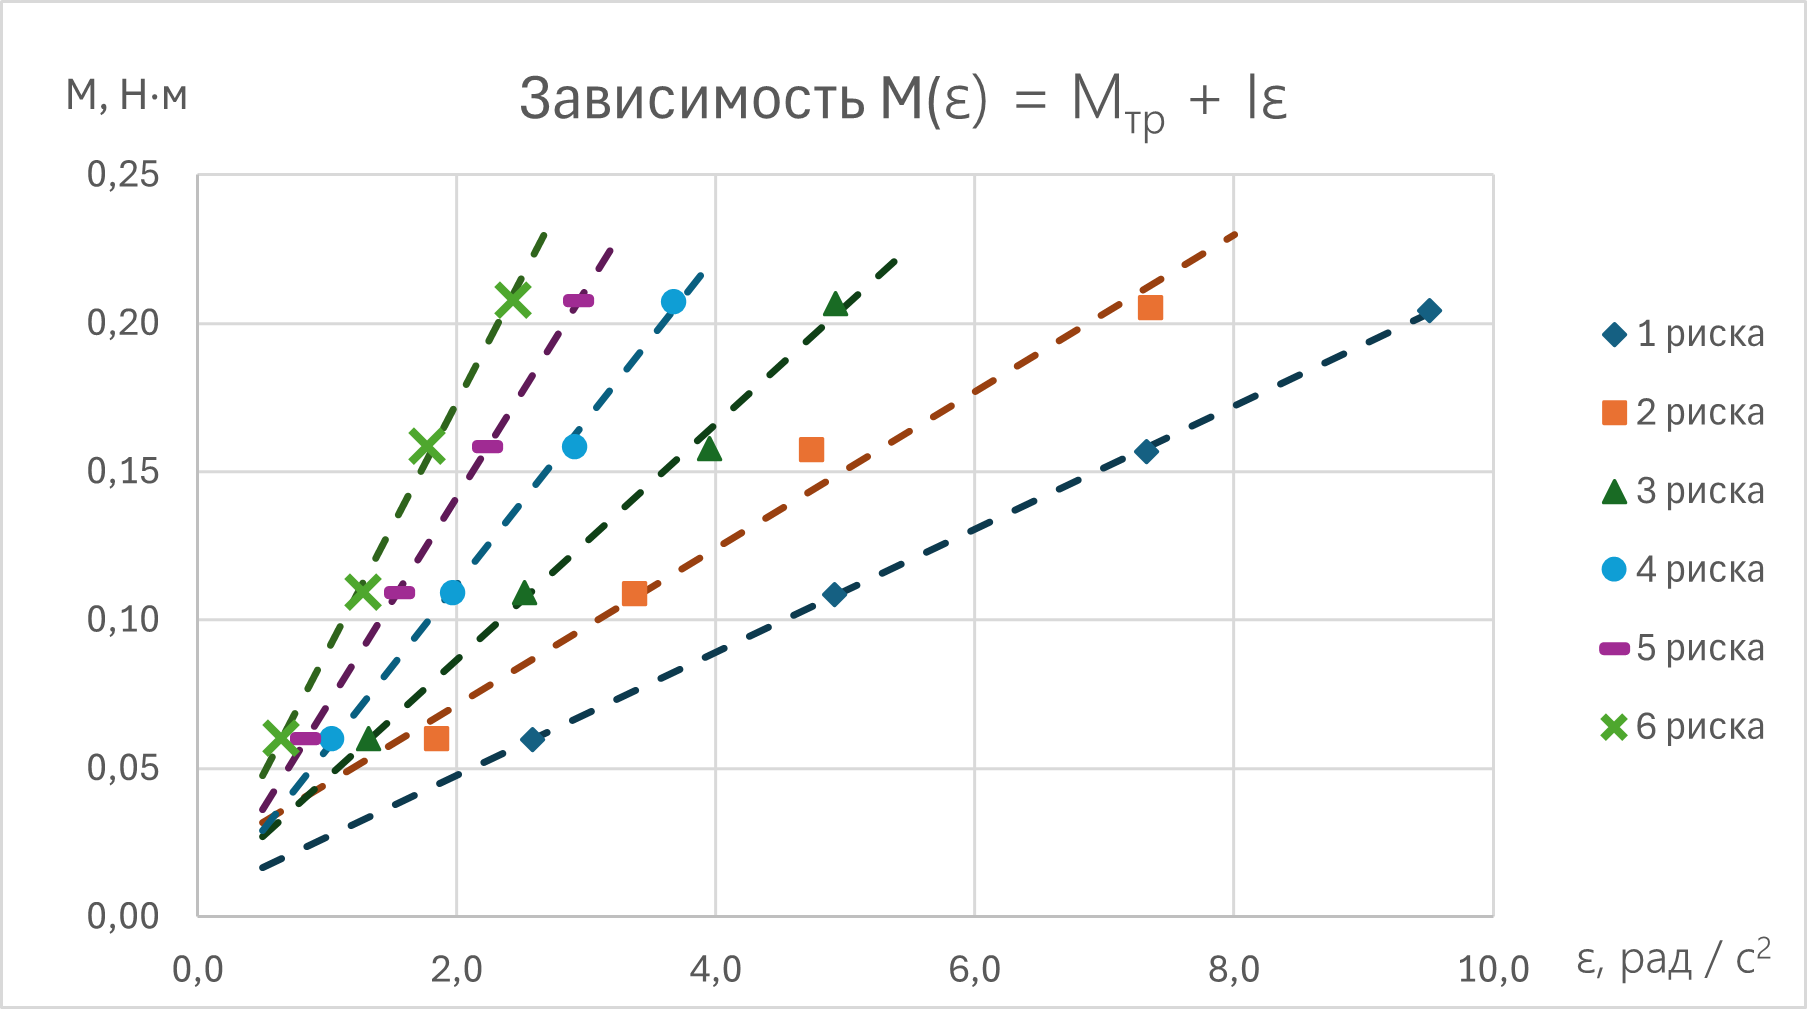
\includegraphics[width=15cm]{images/diagram1}

    \smallvspace

    \textit{График 1.} Зависимость $M(\varepsilon) = M_\text{тр} + I\varepsilon$
\end{center}

\begin{center}
    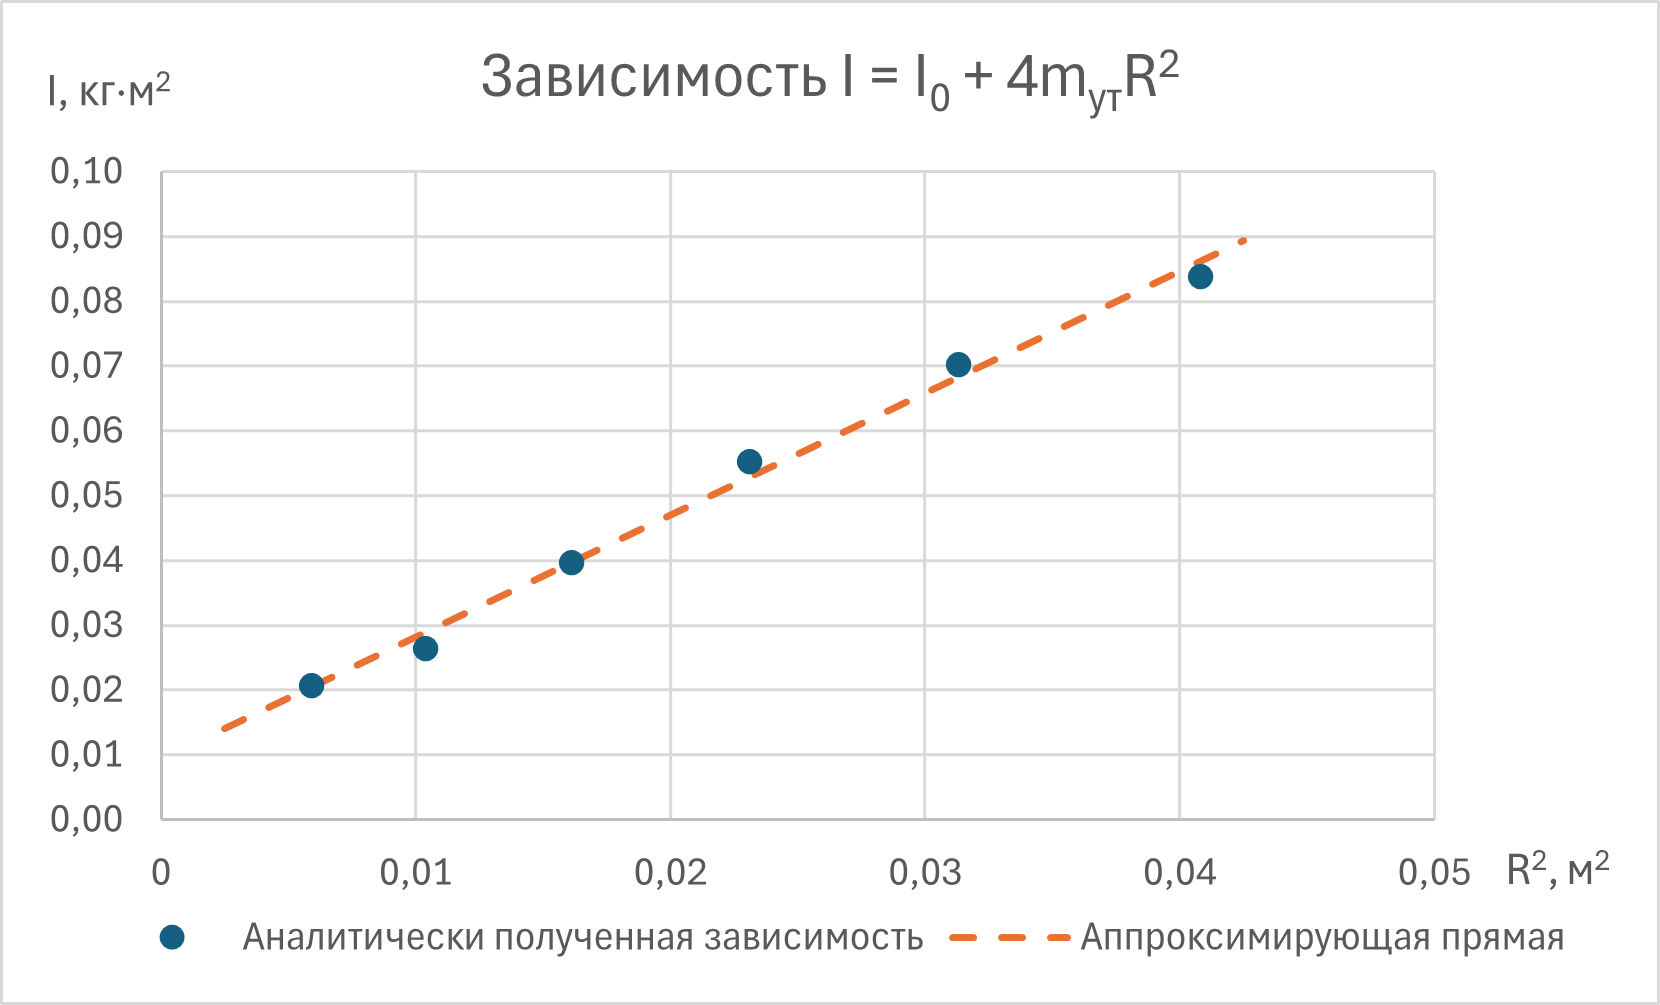
\includegraphics[width=15cm]{images/diagram2}

    \smallvspace

    \textit{График 2.} Зависимость $I = I_0 + 4m_\text{ут} R^2$
\end{center}



\end{document}